\section{The Large Hadron Collider}\label{sec:lhc}

The Large Hadron Collider (LHC) at the European Organisation for Nuclear Research (CERN), in Geneva, Switzerland is the highest-energy particle accelerator constructed to date. 
It is designed to operate at a centre of mass (CoM) energy of 14\TeV, through two 7\TeV proton beams travelling in 2808 bunches of up to $1.15 \times 10^{11}$ protons at a collision rate of 25\nsm which corresponds to a design luminosity of $10^{34}\percms$. 
The LHC can also operate in a heavy-ion mode, where lead ions are collided at 2.76\TeV per nucleon usually for one month a year~\cite{Bayatian:2006zz}.

The beams collide at four interaction points around the LHC, with one of the four major experiments being based at each of them. 
The experiments are: A Toroidal LHC Apparatus (ATLAS) and the Compact Muon Solenoid (CMS) detectors, which are the two multi-purpose experiments; the Large Hadron Collider beauty (LHCb) is an experiment which specialises in b-physics and; A Large Ion Collider Experiment (ALICE), as the name suggests, specialises in heavy ion physics~\cite{Bruning:782076}. 

\subsection{Motivation}
The core motivations behind the LHC are to shed light on the nature of the electroweak symmetry breaking, which the Higgs was presumed and found to be responsible, and to probe the consistency of the SM above the \TeV level through precision measurements of SM parameters and the Higgs mechanism.
Alternative theories to the SM, such as SUSY theories, additional dimensions or new fundamental forces and particles are expected to emerge at the TeV level, giving the potential to ascertain whether these theories have any basis beyond mere conjecture.
The primary motivation behind operating the LHC in a heavy-ion mode is to search for evidence of the plasma of quarks and gluons, which is made possible through the resultant production of QCD matter under extreme temperature, density and low momentum fractions of partons~\cite{Baur:687318}.

\subsection{Accelerator Complex}
When operating in proton-proton mode, the preparation of the beams starts at Linear accelerator 2 (Linac2). 
Protons from a hydrogen gas source are accelerated to 50\MeV and are injected into the Proton Synchrotron Booster which accelerates the protons to 1.4\GeV before injection into the Proton Synchrotron (PS). 
In the PS, the protons are accelerated to 26\GeV and are injected into the Super Proton Synchrotron (SPS) where they are accelerated to 450\GeV before finally entering the LHC~\ref{fig:cern-accelerator-complex}. 
When operating with lead ions, Linear accelerator 3 (Linac3) is used to initially accelerate the ions before injecting them into the Proton Synchrotron Booster, before the ions use the same accelerators as the protons do to prepare them for use in the LHC\~cite{Bruning:782076}. 

The LHC beam requires 1232 dipole magnets to bend the beam along its circular path and 392 quadrupole magnets to focus the beams, with each magnet producing a 8.3T field whilst operating at 1.9K.
Sixteen Radio Frequency (RF) cavities (eight per beam) are used to accelerate the beams up to their designed operational energies of 7\TeV over the course of circa twenty minutes. 
Each cavity operates at frequency of 400\MHz, at a temperature of 4.5K, delivering a maximum of 2 MV. 
The charged particles which pass through the cavities are accelerated by the energy imparted by the resonant electromagnetic field. 
If a charged particle arrives out of synchronisation with the operational frequency, such particles are either accelerated or decelerated so that they stay close to the energy of the ideal particle. 
This results in the charged particles being grouped into bunches before magnets near each of the four interaction points bend the beams so that they collide in the heart of the four main detectors.
A more detailed description of the LHC accelerator chain at CERN can be found in~\cite{Schindl:397574}. 

\begin{figure}[htbp]
\begin{center}
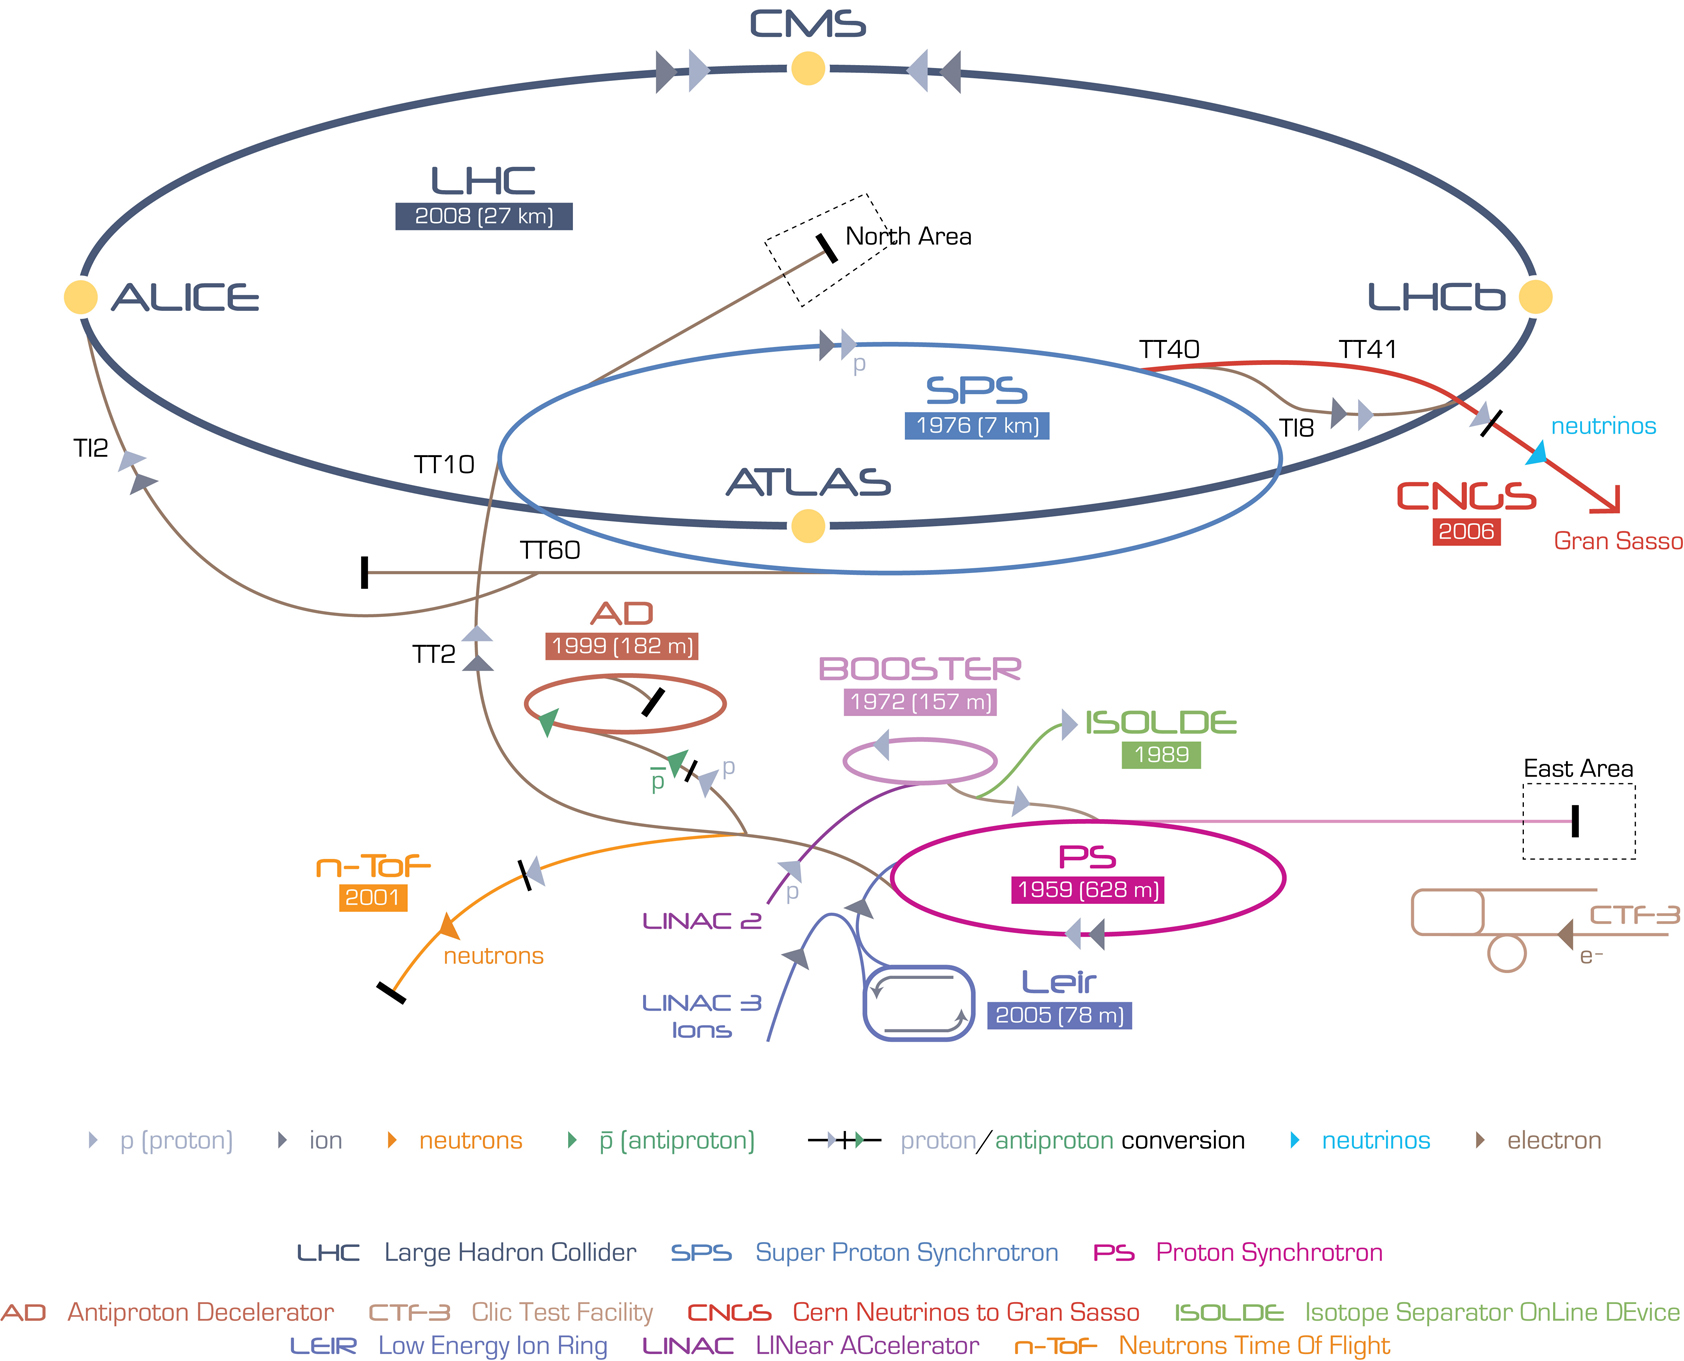
\includegraphics[width=0.97\textwidth]{figs/lhc/Cern-Accelerator-Complex.jpg}
\caption{CERN complex, including the various linear accelerators, synchrotrons, LHC, LHC detectors and other aspects of the complex.}
\label{fig:cern-accelerator-complex}
\end{center}
\end{figure}
